% Information architecture of the TERRA studio mode.
%
% Records the scientific premise of the studio, the measured pressure its
% analyses place on screen space, and a reference architecture drawn from
% Blender. Written because the reasoning is not recoverable from the code:
% the code shows what was built, not which question it answers.
%
% Build:  latexmk -pdf studio_information_architecture.tex
\documentclass[11pt,a4paper]{article}

\usepackage[T1]{fontenc}
\usepackage[utf8]{inputenc}
\usepackage[english]{babel}
\usepackage{lmodern}
\usepackage{microtype}
\usepackage[margin=2.6cm]{geometry}
\usepackage{amsmath,amssymb}
\usepackage{booktabs}
\usepackage{longtable}
\usepackage{graphicx}
\usepackage{pgfplots}
\pgfplotsset{compat=1.17}
\usepackage{tikz}
\usetikzlibrary{positioning,arrows.meta,fit,backgrounds}
\usepackage{caption}
\captionsetup{font=small,labelfont=bf}
\usepackage[hidelinks]{hyperref}
\usepackage{enumitem}
\setlist{itemsep=2pt,parsep=0pt}

\newcommand{\code}[1]{\texttt{\small #1}}

\title{Information Architecture of the TERRA Studio Mode:\\
Evaluating a Land-Cover Model Across Domains}

\author{Jo\~ao Leonardi\textsuperscript{a}}
\date{}

\begin{document}

\maketitle

\begin{center}
\small\textsuperscript{a}Computer Vision Research Center, iCEV Institute of
Higher Education, Teresina, Brazil.
\end{center}

\begin{abstract}
\noindent
The TERRA studio is a WebGL surface that detaches analysis rasters from
geographic coordinates so that several areas of interest (AOIs) can be read
together. This document records why that surface exists, what scientific
question it is built to answer, and the constraint that follows from the
answer. The question is model transferability: given a classifier fitted on one
region, how does its accuracy behave on regions it was not fitted on, and is
the degradation attributable to distributional shift. That question imposes a
\emph{star} topology --- one privileged reference domain against $N$ target
domains --- rather than the pairwise topology the interface was first built
for, and the distinction is not cosmetic: pairwise devices scale as
$\binom{N}{2}$ while the analysis itself scales as $N$. A static audit of the
result payload found approximately 822 transitively declared fields, of which
the studio surfaces on the order of 60 to 70; three quantities computed by the
sidecar are dropped in transit and cannot reach any surface, including the
per-feature table that localises distributional distance to named features. Two
constraints bound any response and are measured here: the application's minimum
window of $1000 \times 700$ pixels, at which existing chrome already consumes
half the width, and the fact that the editors a first reading would propose
building already exist as separate screens. Blender is examined as a reference
architecture for dense professional interfaces, with mechanisms separated into
those that transfer and those that do not, and supplemented from scientific
visualisation where Blender is silent --- notably on what makes two measured
rasters comparable at all. Limitations are stated in
Section~\ref{sec:limitations}.
\end{abstract}

\section{Scope and purpose of this document}

The studio was built incrementally, and its surfaces --- an outliner column, a
selection column, a detail band, a run band, two modal dialogs --- were each
added to answer a local need. The code records what was built. It does not
record which scientific question the arrangement serves, and without that
record the arrangement cannot be evaluated, only adjusted.

This document states the question, derives the information structure it
implies, measures the gap between that structure and the current interface, and
describes a reference architecture. It is a design record, not an
implementation plan.

\section{The scientific premise}

\subsection{The evaluation scenario}

A land-cover classifier is fitted on labelled samples drawn from one region.
The operational question is whether it can be applied elsewhere. In TERRA this
is asked concretely: an AOI is imported on the map, a run is executed, and the
result is brought into the studio. Repeating this for regions that differ from
the training region --- in phenology, soil background, cloud regime, crop
calendar and sensor viewing geometry --- produces a set of results that are
comparable in structure and different in provenance.

A representative case: a model fitted in the Brazilian Northeast, then applied
in the South, the North and the West. Each target region carries different
spectral and phenological characteristics. The number of AOIs is not bounded by
the method; it is bounded by how many regions the analyst chooses to test.

\subsection{The topology is a star, not a graph}

The set of AOIs is not symmetric. One of them --- the training region --- is
privileged, and every other is measured against it. Comparisons among the
target regions are defined but do not answer the question being asked.

For $N$ AOIs this is the difference between $N-1$ meaningful comparisons and
$\binom{N}{2}$ possible ones. With $N=6$: five comparisons carry the analysis,
and fifteen pairs exist. An interface whose primary comparison device is
pairwise therefore presents ten arrangements that answer nothing, and requires
$N-1$ separate invocations to assemble the answer it does support.

\begin{figure}[t]
\centering
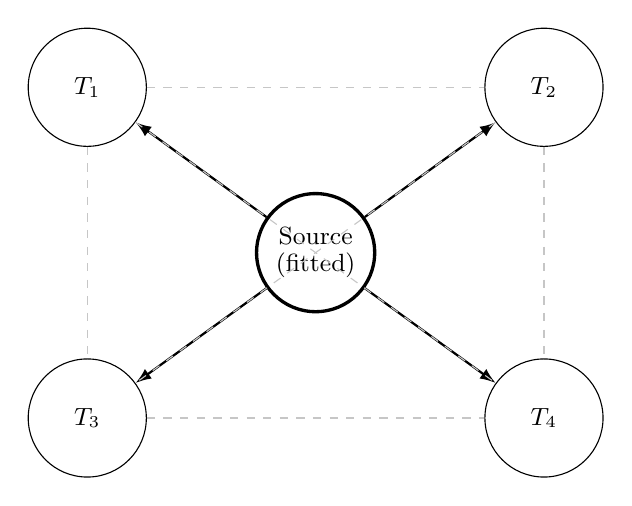
\begin{tikzpicture}[
  dom/.style={circle,draw,minimum size=1.5cm,inner sep=1pt,font=\small},
  ref/.style={dom,very thick},
  edge/.style={-{Latex[length=2mm]},thick},
  faint/.style={gray!45,thin,dashed}
]
\node[ref] (S) at (0,0) {\shortstack{Source\\(fitted)}};
\node[dom] (A) at (-2.9,2.1) {$T_1$};
\node[dom] (B) at (2.9,2.1) {$T_2$};
\node[dom] (C) at (-2.9,-2.1) {$T_3$};
\node[dom] (D) at (2.9,-2.1) {$T_4$};
\foreach \t in {A,B,C,D} \draw[edge] (S) -- (\t);
\draw[faint] (A) -- (B); \draw[faint] (A) -- (C); \draw[faint] (A) -- (D);
\draw[faint] (B) -- (C); \draw[faint] (B) -- (D); \draw[faint] (C) -- (D);
\end{tikzpicture}
\caption{Comparison topology for $N=5$. Solid arrows are the $N-1$ comparisons
the transferability question defines; dashed edges are the remaining
$\binom{N}{2}-(N-1)$ pairs, which are computable and do not bear on it. A
pairwise comparison device does not distinguish between the two kinds.}
\label{fig:star}
\end{figure}

\subsection{Why the shift is not covariate shift}

Land cover is anticausal in the sense of Sch\"olkopf et al. (2012): the class
generates the observed reflectance, not the reverse. Covariate shift assumes
$P(Y \mid X)$ is stable while $P(X)$ moves, which is the causal direction and
does not hold here. What moves between regions is the class prior $P(Y)$ ---
crop composition differs --- together with the class-conditional appearance
$P(X \mid Y)$, since the same crop presents differently under a different soil
background and calendar. This combination is generalized target shift in the
sense of Zhang et al. (2013), and it is the regime the studio's diagnostics
must describe.

\subsection{The figure the question resolves to}

Ben-David et al. (2010) bound the target error of a hypothesis $h$ by
\begin{equation}
\varepsilon_T(h) \;\le\; \varepsilon_S(h)
\;+\; d_{\mathcal{H}\Delta\mathcal{H}}(\mathcal{D}_S,\mathcal{D}_T)
\;+\; \lambda ,
\label{eq:bound}
\end{equation}
where $\varepsilon_S$ is the source error, $d_{\mathcal{H}\Delta\mathcal{H}}$ a
divergence between the two marginals, and $\lambda$ the error of the best joint
hypothesis. The bound states that divergence constrains the error gap. It does
not state that the constraint is tight, and whether it is tight for a given
model and sensor is an empirical question.

That question is answered by plotting divergence against observed accuracy for
all $N$ AOIs at once (Figure~\ref{fig:scatter}). Each AOI contributes one
point. Three readings follow directly from the arrangement:

\begin{itemize}
\item Points falling near a descending trend indicate that divergence accounts
      for the observed degradation, and the bound in Eq.~\eqref{eq:bound} is
      informative for this model.
\item A point at large divergence and high accuracy indicates transfer despite
      distance, which suggests the divergence measure is capturing variation
      the classifier is invariant to.
\item A point at small divergence and low accuracy indicates that the cause is
      elsewhere --- label definitions, reference quality, spatial resolution,
      or the $\lambda$ term --- and not distributional distance.
\end{itemize}

\begin{figure}[t]
\centering
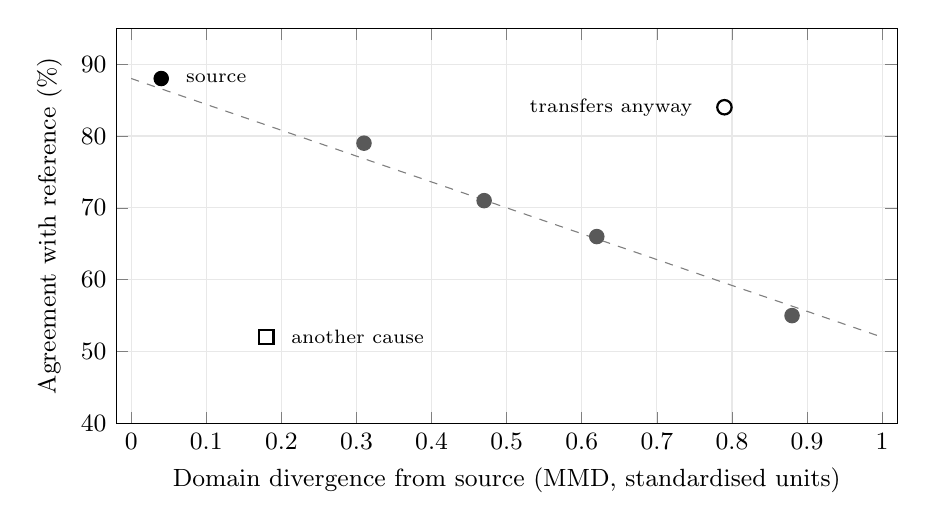
\begin{tikzpicture}
\begin{axis}[
  width=11.5cm, height=6.6cm,
  xlabel={Domain divergence from source (MMD, standardised units)},
  ylabel={Agreement with reference (\%)},
  xmin=-0.02, xmax=1.02, ymin=40, ymax=95,
  grid=major, grid style={gray!18},
  tick label style={font=\small}, label style={font=\small},
  every axis plot/.append style={mark size=2.6pt},
]
\addplot[only marks,mark=*,black] coordinates {(0.04,88)};
\addplot[only marks,mark=*,gray!70!black] coordinates {
  (0.31,79) (0.47,71) (0.62,66) (0.88,55)};
\addplot[only marks,mark=o,black,thick] coordinates {(0.79,84)};
\addplot[only marks,mark=square,black,thick] coordinates {(0.18,52)};
\addplot[dashed,gray,domain=0:1,forget plot] {88 - 36*x};
\node[font=\scriptsize,anchor=west] at (axis cs:0.06,88) {source};
\node[font=\scriptsize,anchor=east] at (axis cs:0.76,84) {transfers anyway};
\node[font=\scriptsize,anchor=west] at (axis cs:0.20,52) {another cause};
\end{axis}
\end{tikzpicture}
\caption{Divergence against accuracy, one point per AOI. Illustrative values,
not measurements. The arrangement is the analysis rather than a summary of it:
the trend tests whether Eq.~\eqref{eq:bound} is tight for this model, and the
two annotated outliers are the cases worth investigating. The figure scales
linearly in the number of AOIs.}
\label{fig:scatter}
\end{figure}

This is one figure with $N$ points, and it is the deliverable of the
transferability study. The studio does not currently produce it.

\section{Measured pressure on the interface}

\subsection{Field count, and what it does and does not mean}

A static traversal of \code{PredictResult} and its transitive members in
\code{frontend/src/lib/types.ts} reaches approximately 822 declared fields. The
studio reads on the order of 60 to 70 of them. Three whole product payloads,
accounting for roughly 576 fields, have no studio surface.

This figure is easy to misread and the qualification matters. Those payloads are
\emph{not} unrendered by the application: \code{pages/AnalysisPage.tsx} mounts
\code{WindScreening}, \code{EnergyModelSection}, the solar resource, terrain and
siting sections and \code{LulcSection}, each gated on the presence of its
payload rather than greyed out when absent --- which is already the discipline
described in Section~5.4. The application renders them; the studio does not.

The number therefore measures one thing only: how much of a result is outside
the studio's reach, and so how much a multi-AOI comparison performed there
cannot consult. It is not evidence of a missing feature elsewhere.

\subsection{Surfaces that already exist}
\label{sec:existing}

A design record that proposes building what is already built is worse than no
record. Four components bear directly on the proposals in Section~6 and are
present in the codebase:

\begin{itemize}
\item \code{frontend/src/components/DataTableView.tsx} renders a sortable table
      with missing-value-last ordering, clipboard copy and CSV download.
\item \code{frontend/src/lib/analysisTables.ts} exports on the order of 28 table
      builders keyed on payload presence, among them
      \code{domainFingerprintTable}, \code{lulcPredVsRefTable} and the
      wind and energy families.
\item \code{ResearchPackModal} lists every table a result carries with its row
      count, named after the files the exporter writes, so an inspection maps
      one-to-one onto the exported pack.
\item \code{frontend/src/components/whiteboard/boardMemory.ts} is a
      module-scoped keyed record that outlives component remounts, holding
      per-slot state across a visit to another screen.
\end{itemize}

The tabular capability described in Section~6.2 therefore exists as a
\emph{component} and is absent as a \emph{studio surface}. What is missing is
the routing, not the table.

\code{boardMemory} additionally records a deliberate position that one proposal
below contradicts: its documentation states that it is not persistence, that it
survives a close and not a restart, and that saving is something a user asks for
by name. Any proposal to persist disclosure state is a reversal of that
decision and must be argued against it rather than presented as filling a gap.

\subsection{Quantities computed and then dropped}

Three outputs of \code{sidecar/domain\_shift.py} are not carried through the
Go type that declares the report, and therefore cannot reach the interface at
all. Each is load-bearing for the interpretation of the others.

\begin{itemize}
\item \code{feature\_shift} --- a per-feature table giving, for the twelve
      features with the largest displacement, the standardised means in each
      domain, the gap in training standard deviations, and the classifier's
      impurity importance. A scalar divergence states that two domains differ;
      this table states \emph{where}. Without it a large distance is not
      actionable.
\item \code{same\_space} and \code{standardised} --- qualifiers stating whether
      two fingerprints are comparable at all. Comparing an 80-feature spectral
      fingerprint against a single-column NDVI fingerprint produces a number
      from two different quantities. Without these flags every distance shown
      is unqualified.
\item \code{cva\_magnitude\_sd} --- change-vector magnitude expressed in
      training standard deviations. The interface currently shows the raw
      magnitude. Measured on the shipped artifacts, six acquisition-index
      features account for 99.7\% of the raw squared distance while the sixteen
      reflectance features account for the remainder, so the raw figure is
      dominated by quantities that carry no domain meaning. Standardising moved
      one reflectance shift from a factor of 1.4 to 5.5.
\end{itemize}

\subsection{The geometric budget}
\label{sec:budget}

Any proposal that adds or widens a surface is bounded by a figure that is set in
the application and not negotiable at the level of a stylesheet:
\code{app.go} sets a minimum window of $1000 \times 700$ pixels.

At that minimum the two columns consume $240 + 255 = 495$\,px, which is
49.5\,\% of the width, and the two foot bands consume 212\,px of 700, which is
30.3\,\%. The canvas the studio exists to present therefore receives
approximately $505 \times 488$\,px --- under a quarter of the window area.

Table~\ref{tab:budget} gives the consequence for one concrete proposal. The
reference legend names 17 cover classes, so a confusion matrix over them, at a
cell size that can be read, requires on the order of 500\,px of width. Seating
that in a widened right column at the minimum window leaves roughly 260\,px of
canvas between the two columns.

\begin{table}[h]
\centering
\small
\caption{Width budget at the minimum window of 1000\,px.}
\label{tab:budget}
\begin{tabular}{@{}lrr@{}}
\toprule
& As built & With a 500\,px matrix column \\
\midrule
Left column   & 240\,px & 240\,px \\
Right column  & 255\,px & 500\,px \\
Canvas        & 505\,px & 260\,px \\
\midrule
Canvas share  & 50.5\,\% & 26.0\,\% \\
\bottomrule
\end{tabular}
\end{table}

The budget is the reason the arrangement cannot be resolved by making surfaces
larger. Screen area is fixed; only its allocation over time is free, which is
the argument for task-bound layouts in Section~\ref{sec:transfers} and against
adding permanent chrome.

\section{Current surfaces}

Table~\ref{tab:surfaces} records the studio as built, from a static read of
\code{BoardSurface.tsx} and \code{MapScreen.tsx}.

\begin{table}[t]
\centering
\small
\caption{Reading and input surfaces of the studio. Widths are the values in the
source; the two columns and the run band are unconditional.}
\label{tab:surfaces}
\begin{tabular}{@{}llll@{}}
\toprule
Surface & Kind & Extent & Carries \\
\midrule
\code{BoardSidebar}      & column & 15\,rem, left        & scene tree, data, areas \\
\code{BoardStatsBar}     & column & 15.94\,rem, right    & one plane: legend, accuracy \\
\code{BoardSolarDetail}  & band   & foot, 1.25--22\,rem  & two planes: delta, transitions \\
\code{BoardRunBar}       & band   & foot, 4\,rem         & run parameters (input) \\
\code{BoardCompareModal} & modal  & covers the view      & swipe, domain shift, matrices \\
\code{BoardAreaModal}    & modal  & covers the view      & polygon drawing (input) \\
\code{boardScene}        & canvas & full, beneath        & the rasters themselves \\
\bottomrule
\end{tabular}
\end{table}

Two properties of this arrangement bear on the premise in Section~2.

\paragraph{The detail band is defined only for two planes.} It mounts when the
selection path contains exactly two predictions. For one plane it does not
mount; for three or more, the expression that selects ``the two'' is not
defined by the analysis. The rule that assigns content to surfaces by
\emph{arity} --- one plane to the column, two to the band --- is well defined
at $N \le 2$ and undefined above it.

\paragraph{Both modal dialogs require covering the 3D view.} Drawing an area
and comparing two rasters are each implemented as a full-screen scrim. The
comparison is opened by a gesture performed \emph{on} the board, and its result
hides the board that gesture referred to.

\section{Blender as a reference architecture}

Blender is examined because it is a mature interface for a professionally dense
task, in continuous use and revision for approximately three decades, with its
design rules stated explicitly rather than inferred.

\subsection{Non-overlap as a data-model invariant}

Blender's Human Interface Guidelines state the rule directly: the interface
should present the relevant options ``at a glance, without the need for pushing
or dragging windows around,'' for which reason it defaults to a subdivided
window layout. The subdivision operates on three levels: \emph{Screens} (the
whole layout), \emph{Areas} (containers), and \emph{Regions} (header, toolbar,
sidebar, footer, main region inside an editor).

The mechanism is stronger than the guideline. Each area holds four corner
vertices that are shared with its neighbours, so resizing moves a shared edge
and neighbouring areas follow by construction. Overlap is not discouraged by
convention; it is unrepresentable in the structure. A rule enforced by the data
model cannot erode through incremental change, which is the relevant property
for a long-lived interface.

\subsection{Areas, editors and workspaces}

Any area can host any editor type, and the state of every editor that has
occupied a given area is retained, so switching type is reversible without loss.
Workspaces are named layouts --- eleven ship by default, among them Layout,
Modeling, Sculpting, Shading, Animation, Compositing and Geometry Nodes --- each
a saved arrangement of areas and editors bound to a task.

This is the mechanism most relevant to the trade-off that motivated this
document. Blender's response to information density is not to display more
simultaneously; it is to make the arrangement a property of the task and let
the user switch. Tools for sculpting are not on screen while animating, and
their absence is not a limitation but the design.

A second mechanism relaxes the tiling temporarily rather than permanently: an
area can be maximised to the whole window and restored, and a subset of objects
can be isolated in the viewport. Both give one surface the full window without
introducing an overlapping layer, so the state remains a property of the
partition and is reversible by the same gesture that produced it. This is what
the guidelines offer in place of a dialog when a task genuinely needs the whole
screen.

\subsection{Pinning, and comparison without a dialog}

Editors follow the active selection by default, which is what allows one surface
to serve many purposes. Pinning breaks that link on demand: a pinned properties
editor continues to display the object it was pinned to while the selection
moves elsewhere.

The consequence is a general substitute for a comparison dialog. Two editors,
each pinned to a different subject, placed side by side by subdivision, compare
those subjects without concealing anything and without a device built for the
purpose. The mechanism generalises past two --- $k$ pinned editors compare $k$
subjects --- and it composes with the aggregate view rather than replacing it.

\subsection{Context sensitivity}

Panels resolve their contents through an ordered chain rather than from global
state: the layout context is consulted first, then the region, then the area,
then the screen. Consequently one physical surface serves many purposes without
configuration --- the Properties editor changes its tab set with the active
object, and the sidebar shows properties of the active item. Pinning exists as
an explicit escape from this coupling when a panel must stop following the
selection.

\subsection{Devices for density}

Recurring mechanisms, applied consistently across editors:

\begin{itemize}
\item A scope selector that re-lenses one widget onto different slices of the
      data model (the Outliner's display modes: View Layer, Scenes, Blender
      File, Data API, Library Overrides, Unused Data).
\item A filter popover cutting on structural and state axes rather than name,
      with an invert toggle that doubles every state filter.
\item Per-row state columns --- visibility, selectability, renderability ---
      with modifier keys for subtree propagation, so the state of hundreds of
      objects is legible in one icon grid.
\item Graded expansion operators, from a single row to the whole tree, so row
      count is a dial rather than a consequence.
\item Panels and sub-panels as progressive disclosure, with disclosure state
      saved in the document rather than reset per session.
\item Search that dims non-matching entries and switches tabs, instead of
      reducing the view to a filtered list.
\item An \emph{Operate then Settings} pattern: an operator runs immediately with
      previous settings and exposes an adjustable region afterwards, replacing
      the pre-flight parameter dialog.
\item The Spreadsheet editor, introduced in version 2.93, presenting per-element
      data as a filterable table.
\end{itemize}

\section{Correspondence and its limits}

\subsection{Structural correspondence}

The studio arrived independently at an arrangement close to Blender's, which
suggests the arrangement is a response to the shape of the problem rather than
to a particular tradition.

\begin{table}[h]
\centering
\small
\caption{Correspondence between studio surfaces and Blender editors.}
\label{tab:map}
\begin{tabular}{@{}lll@{}}
\toprule
Studio & Blender & Correspondence \\
\midrule
\code{boardScene}        & 3D Viewport            & direct \\
\code{BoardSidebar}      & Outliner               & direct; lacks per-row state columns \\
\code{BoardStatsBar}     & Sidebar (N) / Properties & direct; not context-routed by tabs \\
\code{BoardSolarDetail}  & horizontal editor at the foot & partial \\
\code{BoardRunBar}       & tool header / tool settings & direct \\
\code{BoardCompareModal} & \emph{none}            & no counterpart \\
\code{BoardAreaModal}    & \emph{none}            & no counterpart \\
\bottomrule
\end{tabular}
\end{table}

The two rows without counterparts are the two modal dialogs. Blender's answer to
a comparison task is to subdivide the workspace so both subjects remain visible,
which is the same operation the studio performs conceptually when it lifts two
rasters onto one surface --- and then abandons by opening a dialog over them.

\subsection{The studio is one editor, not the container}
\label{sec:oneeditor}

The correspondence in Table~\ref{tab:map} invites a reading that should be
stated and rejected: that the studio is Blender's window and its surfaces are
Blender's editors, so anything missing must be added \emph{inside} the studio.

Blender does not resolve a demand for tabular data by extending the 3D
Viewport's sidebar. It gives an area a different editor type. The
correspondence therefore runs one level up: the studio is \emph{an editor}, and
the application already has others. \code{pages/AnalysisPage.tsx} carries the
figures, tables and the research pack; \code{CompareAnalyses.tsx} carries
side-by-side comparison including the domain-shift section, phenology series
and class statistics.

What the application lacks is not those editors. It is that they are
\emph{screens} --- navigated between, one at a time, mutually exclusive ---
rather than \emph{editors} that can occupy areas of one partition. Under
Blender's model, examining a raster in the studio while its tables stand open
beside it is an ordinary arrangement; here it requires leaving one screen for
another.

This reading also disposes of a proposal the analysis initially favoured.
Adding a tabular pane to the studio would create a third comparison surface
alongside the studio's own and \code{CompareAnalyses}, with no account of which
is authoritative when they disagree. The transfer that follows from the analogy
is to make the existing editors tileable, not to grow one of them.

\subsection{Mechanisms that transfer}
\label{sec:transfers}

\begin{enumerate}
\item \textbf{Comparison by subdivision and pinning rather than by dialog.}
      Removes the contradiction of a comparison hiding its own subjects, and
      admits $N > 2$ without redefinition: $k$ pinned surfaces compare $k$
      subjects. Where a task needs the whole window, maximising an area supplies
      it without an overlapping layer.
\item \textbf{Task-bound layouts.} Classification, comparison and diagnosis
      place different demands on the same space. Domain-shift diagnosis is a
      distinct task and need not share a layout with classification.
\item \textbf{Context routing of the selection column.} Replaces the arity rule
      with a mechanism that does not break at $N = 3$: the column shows the
      active item, and the aggregate view shows the set.
\item \textbf{A tabular surface for per-element data.} One row per AOI, sortable
      by divergence, accuracy, quantity and allocation disagreement. This is the
      surface Figure~\ref{fig:scatter} selects from, and the natural home for
      the fields listed in Section~3.2. As Section~\ref{sec:existing} records,
      the table component and its builders already exist; what is absent is a
      studio surface that routes to them.
\end{enumerate}

\subsection{A precondition the correspondence does not supply}
\label{sec:precondition}

Replacing the comparison dialog with pinned side-by-side surfaces carries a
requirement that Blender does not raise, because Blender's editors compare
objects and not measured fields.

Two rasters are not comparable by eye unless they share a colour mapping. A
continuous layer whose ramp is rescaled to its own range, placed beside another
rescaled to its own, will present two different values in the same colour and
two equal values in different colours. The reading is confident and wrong, which
is a worse failure than the dialog it replaces, since the dialog at least
prevented the comparison from being attempted casually.

The mechanism this needs is not in Blender. It is in scientific visualisation:
ParaView separates the colour transfer function from the view and exposes
explicit rescaling --- to the data range, to a custom range, or to the range
over all timesteps --- so that a shared mapping is a stated choice rather than a
side effect. Any side-by-side arrangement in the studio requires an equivalent:
one legend domain, reconciled across the panes, with the reconciliation visible.

\subsection{Mechanisms that do not transfer}

\begin{itemize}
\item \textbf{General-purpose editors.} Blender's editors are general: a graph
      editor edits any animatable value. The studio's surfaces are specific to
      the structure of a run, and a panel that is empty for a single AOI is not
      an editor in Blender's sense.
\item \textbf{The learning investment.} Blender's interface is oriented to
      practitioners who use it for years, and its learning curve is a documented
      and frequently reported cost. Adopting its flexibility adopts part of that
      cost. The studio's audience is stated as research-level analysis, which is
      a comparable profile, but the trade-off is a choice rather than a
      consequence.
\item \textbf{Absence of long-running jobs.} A TERRA run is asynchronous,
      remote and may fail. Blender's closest analogue is rendering, which is
      handled by a dedicated editor rather than by the general layout mechanism,
      so the run band has no direct counterpart to inherit from.
\end{itemize}

\section{References outside Blender}

Blender answers the layout question well and is silent on several requirements
specific to measured data. Three other mature applications supply mechanisms
that Blender has no reason to have.

\paragraph{ParaView.} Views are first-class occupants of the tiled partition ---
render view, spreadsheet view, line chart, parallel coordinates --- and the same
source can be shown in several view types at once with \emph{linked selection}
between them, so selecting rows in the spreadsheet highlights the corresponding
elements in the 3D view. This is a closer fit than Blender's editor-as-slot for
the case in Section~2, where one set of AOIs must be read as a scatter, as a
table and as rasters simultaneously. Two further devices apply directly: the
colour transfer function is decoupled from the view with explicit rescaling
(Section~\ref{sec:precondition}), and visibility in the pipeline browser is
scoped to the active view rather than global, which is what a multi-pane
arrangement requires and Blender's single global outliner toggle cannot express.
ParaView's Information panel is also a schema-driven readout of the active
source's arrays, ranges and element counts, defined over the data model rather
than per payload --- a low-cost route to a large field count that needs no pane
type per product.

\paragraph{QGIS.} The Processing History panel records every algorithm
invocation with its complete parameter dictionary, re-runnable from the record,
alongside batch processing over many inputs. This is the provenance and
repeatability device for expensive asynchronous operations, which is TERRA's
cost model and is precisely where Blender's \emph{Operate then Settings} does
not apply --- that pattern is safe only because a Blender operator is cheap to
re-run, and a TERRA run is minutes long and consumes quota. QGIS also ships the
same content as both a docked panel (Layer Styling) and a dialog (Layer
Properties), which is a shipped precedent for the studio's unfinished
\code{placement} distinction.

\paragraph{ImageJ/Fiji.} The ROI Manager makes named regions reusable across any
open image, with measurements appending rows to one cumulative results table.
This makes the region orthogonal to the run: comparing one AOI across $N$
periods becomes $N$ rows in one table rather than $N$ objects on a board, which
bears directly on the saved-area facility recently added. Synchronize Windows
locks pan, zoom and cursor across open images with a shared crosshair, and is
the matured form of the studio's existing link-rasters toggle.

\section{Position as a non-geographic encoding}

The studio's premise is the removal of cartographic coordinates. That removal
frees the coordinate system, and the freed system currently encodes nothing:
planes rest where they were dragged.

A candidate use is to encode domain space --- placing each AOI at the projection
of its feature fingerprint, so that proximity on the board denotes proximity in
feature space and an AOI on which the model fails is visibly separated from the
others. Under this arrangement the spatial structure of the transferability
problem becomes directly observable, which is an operation a cartographic
interface cannot perform, since its coordinates are already committed.

Two constraints apply. Projection from a high-dimensional fingerprint to two or
three dimensions is lossy, and both PCA and t-SNE produce configurations whose
absolute coordinates are not interpretable; relative separation is the only
reading the projection supports, and t-SNE in particular does not preserve
global distances. Second, if position encodes domain then position is no longer
available for manual arrangement, which argues for an explicit arrangement mode
--- manual, domain, geography, accuracy --- rather than a replacement. A mode
selector on a view is the same device as the Outliner's display mode.

\section{Defects observed while preparing this record}

Two are recorded here because they were verified during the audit and are
independent of any proposal above.

\paragraph{The domain-shift report is broken at every link.} The sidecar
defines \code{mmd\_rbf} and emits the key \code{mmd\_rbf}; the Go type declares
\code{MMDLinear} carrying the JSON tag \code{mmd\_linear}; the interface reads
\code{report.mmd\_linear}. The name changed at the source and nothing
downstream followed, so the figure the panel displays cannot be populated. The
sidecar's own test suite calls \code{ds.mmd\_linear}, a function the module no
longer defines, so the tests do not pass either. Separately,
\code{standardised} is derived from the standardised moments \code{z\_mean} and
\code{z\_var}, which the frontend fingerprint type does not carry.

\paragraph{Escape during drawing closes the studio beneath the dialog.} The
modal shell binds no keyboard handler; the studio binds a window-level Escape
that closes it; and the area-drawing dialog is mounted outside the gate that
tracks whether the studio is open. Pressing Escape while drawing therefore
dismisses the surface underneath a dialog that remains on screen.

Both are small and neither is a consequence of the architecture discussed here.
They are noted so that the audit that found them is not lost with it.

\section{Limitations}
\label{sec:limitations}

\begin{itemize}
\item The field counts in Section~3.1 come from a static traversal of type
      declarations. They count declared fields, not fields populated at runtime,
      and optional members are counted once regardless of how often they appear.
\item Figure~\ref{fig:scatter} uses illustrative values. No transferability
      study has been run in TERRA to date, so the relationship between
      divergence and accuracy is not measured here and the figure demonstrates
      an arrangement rather than a result.
\item The divergence measure available in the studio is a maximum mean
      discrepancy with a Gaussian kernel, which is not the
      $d_{\mathcal{H}\Delta\mathcal{H}}$ of Eq.~\eqref{eq:bound}. MMD is used as
      a computable proxy; the substitution is standard practice and is not
      justified by the bound itself.
\item Statements about Blender, ParaView, QGIS and ImageJ describe documented
      behaviour and published guidelines. No user study is cited, and the claim
      that these arrangements work is an argument from adoption and longevity,
      not from measurement.
\item The field counts in Section~3.1 and the budget in Section~\ref{sec:budget}
      were produced by static reading. The budget assumes the minimum window;
      at larger windows the canvas share rises and the constraint relaxes, so
      the figures bound the worst case rather than describing the typical one.
\item The correspondence in Table~\ref{tab:map} is structural. Structural
      similarity does not establish that the mechanisms transfer, which is the
      subject of Section~6.3.
\item No interface change described here has been implemented or evaluated. The
      document records a design position; the position is untested.
\end{itemize}

\section{Summary}

The studio exists to support evaluation of a fitted model on regions it was not
fitted on. That task has a star topology with one privileged source domain, and
it resolves to a single aggregate figure --- divergence against accuracy, one
point per AOI --- that scales linearly in the number of areas examined. The
interface as built is organised around pairwise comparison, which is defined at
$N \le 2$ and undefined above it, and it discards three quantities that qualify
and localise the distances it does display.

Two constraints bound every response. Screen area is fixed by a minimum window
of $1000 \times 700$, at which the existing chrome already takes half the width
and a third of the height, so no arrangement is reachable by enlarging a
surface. And the application already possesses the editors that a first reading
of Blender would propose building: what is absent is that they are exclusive
screens rather than editors that can share one partition.

The central lesson from Blender is accordingly not that density is solved by
displaying more, but that it is managed by binding arrangements to tasks,
routing one surface by context, and subdividing instead of opening a dialog ---
which addresses the studio's one structural contradiction, a comparison that
conceals the subjects it compares. Blender is silent on what makes two measured
rasters comparable at all; that requirement, a shared and explicit colour
mapping, comes from scientific visualisation instead.

\begin{thebibliography}{9}
\small

\bibitem{bendavid2010}
Ben-David, S., Blitzer, J., Crammer, K., Kulesza, A., Pereira, F., \& Vaughan,
J.~W. (2010). A theory of learning from different domains.
\emph{Machine Learning}, 79(1--2), 151--175.

\bibitem{gretton2012}
Gretton, A., Borgwardt, K.~M., Rasch, M.~J., Sch\"olkopf, B., \& Smola, A.
(2012). A kernel two-sample test. \emph{Journal of Machine Learning Research},
13, 723--773.

\bibitem{zhang2013}
Zhang, K., Sch\"olkopf, B., Muandet, K., \& Wang, Z. (2013). Domain adaptation
under target and conditional shift. \emph{Proceedings of the 30th International
Conference on Machine Learning}, 819--827.

\bibitem{scholkopf2012}
Sch\"olkopf, B., Janzing, D., Peters, J., Sgouritsa, E., Zhang, K., \& Mooij, J.
(2012). On causal and anticausal learning. \emph{Proceedings of the 29th
International Conference on Machine Learning}, 1255--1262.

\bibitem{pontius2011}
Pontius, R.~G., \& Millones, M. (2011). Death to Kappa: birth of quantity
disagreement and allocation disagreement for accuracy assessment.
\emph{International Journal of Remote Sensing}, 32(15), 4407--4429.

\bibitem{olofsson2014}
Olofsson, P., Foody, G.~M., Herold, M., Stehman, S.~V., Woodcock, C.~E., \&
Wulder, M.~A. (2014). Good practices for estimating area and assessing accuracy
of land change. \emph{Remote Sensing of Environment}, 148, 42--57.

\bibitem{shneiderman1996}
Shneiderman, B. (1996). The eyes have it: a task by data type taxonomy for
information visualizations. \emph{Proceedings of the IEEE Symposium on Visual
Languages}, 336--343.

\bibitem{tufte1983}
Tufte, E.~R. (1983). \emph{The Visual Display of Quantitative Information}.
Graphics Press, Cheshire, Connecticut.

\bibitem{blenderhig}
Blender Foundation. Human Interface Guidelines --- Paradigms.
\url{https://developer.blender.org/docs/features/interface/human_interface_guidelines/paradigms/}

\bibitem{blendermanual}
Blender Foundation. Blender Manual: Interface --- Window System, Areas, Editors
and Workspaces. \url{https://docs.blender.org/manual/en/latest/interface/}

\bibitem{ahrens2005}
Ahrens, J., Geveci, B., \& Law, C. (2005). ParaView: an end-user tool for large
data visualization. In \emph{The Visualization Handbook}. Elsevier.

\bibitem{paraview}
Kitware. ParaView User's Guide: Views, linked selection, colour maps and
transfer functions. \url{https://docs.paraview.org/}

\bibitem{qgis}
QGIS Development Team. QGIS User Guide: the Processing framework --- history,
batch processing and the Layer Styling panel.
\url{https://docs.qgis.org/latest/en/docs/user_manual/}

\bibitem{schindelin2012}
Schindelin, J., Arganda-Carreras, I., Frise, E., et al. (2012). Fiji: an
open-source platform for biological-image analysis. \emph{Nature Methods},
9(7), 676--682.

\end{thebibliography}

\end{document}
